	\documentclass[twoside]{article}
\usepackage{../../estilo-ejercicios}

%--------------------------------------------------------
\begin{document}

\title{Relación 1}
\author{Javier Aguilar Martín}
\maketitle


\begin{ejercicio}{1.1}
Prueba que todo grafo bipartito de orden $n \geq 3$ es también $r$-partito para $3\leq r \leq n$. ¿Es
cierto el recíproco?
\end{ejercicio}
\begin{solucion}
Sea $G$ un grafo en las condiciones del enunciado. Si $V=V_1\cup V_2$ es la descomposición de $V=V(G)$ como grafo bipartito, basta subdividir $V_1$ y $V_2$ en un total de $r$ subconjuntos disjuntos. Como $n\geq 3$, alguno de los subconjuntos tiene al menos 2 vértices, digamos $V_1$, por lo que podemos subdividirlo en $V_1^1$ y $V_2^1$. Si $n=3$ ya habríamos terminado. Si $n>3$, entonces un subconjunto de entre $V_1^1, V_2^1$ y $V_2$ tiene al menos dos elementos y podemos reiterar el proceso. De este modo, conseguimos que en cada paso sea $r$-partito para un $r$ cada vez mayor, y siempre acotado por $n$, lo cual prueba el resultado. 

El recíproco no es cierto. Por ejemplo en un grafo tripartito completo no podemos unir componentes porque tienen aristas entre ellas, así que no sería bipartito. 
\end{solucion}

\newpage


\begin{ejercicio}{1.2}
Sea $T$ un árbol de orden $p$ que contiene $p_i$ vértices de grado $i$, para cada $i \in\{1,\dots, p-1\}$. Demuestra que $p_1 =
\sum^{p-1}_{i=3} (i - 2)p_i + 2$.
\end{ejercicio}
\begin{solucion}
%Como $T$ tiene orden $p$, $p_{p-1}\in \{0,1\}$. Si $p_{p-1}=1$ entonces todos los demás vértices son hojas conectadas al vértice de grado $p-1$, es decir, $p_1=p-1$ y $p_i=0$ para $1<i<p-1$. Así, la ecuación resultante sería
%\[
%p-1=p-3+2
%\]
%que es trivialmente cierta. Supongamos entonces que $p_{p-1}=0$. 
La ecuación del enunciado se puede reescribir como $\sum_{i=1}^{p-1}(i-2)p_i+2=0$ ya que $p_1$ pasaría a tener coeficiente $-1=1-2$ y $p_2$ tendría coeficiente 0. Ahora la escribimos como
\[
\sum_{i=1}^{p-1} i p_i + 2 = \sum_{i=1}^{p-1}2p_i.
\]
O lo que es lo mismo
\[
\sum_{v\in V(G)}\delta(v)+2=2|V(G)|
\]
Por un lado tenemos que al ser un árbol $|V(G)|=|E(G)|+1$ y por otro tenemos que $\sum_{v\in V(G)}\delta(v)=|E(G)|$ por el lema del apretón de manos, de modo que la igualdad es cierta. 
\end{solucion}

\newpage

\begin{ejercicio}{1.3}

Sea $T$ un árbol de orden $p$ tal que todos sus vértices son de grado 1 o de grado 3. Prueba
que $T$ contiene exactamente $(p - 2)/2$ vértices de grado 3.
\end{ejercicio}
\begin{solucion}
Basta sustituir en la ecuación del ejercicio anterior, que nos daría $-p_1+p_3+2=0$ junto con la condición $p_1+p_3=p$. 
\end{solucion}

\newpage

\begin{ejercicio}{1.4}

Encuentra todos los árboles $T$ tales que su complementario $\overline{T}$ es también un árbol.
\end{ejercicio}
\begin{solucion}

\end{solucion}

\newpage

\begin{ejercicio}{1.5}

Demuestra que todo árbol $T$ tiene un número de hojas mayor o igual que el grado máximo
de $T$.
\end{ejercicio}
\begin{solucion}

\end{solucion}

\newpage

\begin{ejercicio}{1.6}
Prueba que si $G$ es un grafo conexo de orden $p$ tal que todo subgrafo suyo de tamaño
$p -1$ es un árbol ``spanning'', entonces $G$ es un árbol o un ciclo.
\end{ejercicio}
\begin{solucion}
\end{solucion}

\newpage

\begin{ejercicio}{1.7}
Prueba o refuta el siguiente enunciado: Si $G$ es un grafo conexo tal que dos cualesquiera
de sus árboles ``spanning'' son isomorfos, entonces $G$ es un árbol o un ciclo.
\end{ejercicio}
\begin{solucion}

\end{solucion}

\newpage

\begin{ejercicio}{1.8}
Obtén un árbol spanning por el algoritmo DFS del grafo de Grotzsch de la figura adjunta.
\end{ejercicio}
\begin{solucion}





\end{solucion}
\newpage

\begin{ejercicio}{1.9}
Obtén un árbol spanning por el algoritmo DFS del grafo de Petersen de la figura adjunta.
\end{ejercicio}
\begin{solucion}

\end{solucion}
\newpage

\begin{ejercicio}{1.10}
Obtén un árbol spanning por el algoritmo DFS del grafo de Grotzsch de la figura adjunta.
\end{ejercicio}
\begin{solucion}

\end{solucion}

\newpage

\begin{ejercicio}{1.11}
Obtén un árbol spanning por el algoritmo BFS del grafo de Petersen de la figura adjunta.
\end{ejercicio}
\begin{solucion}



\end{solucion}

\newpage

\begin{figure}[h!]
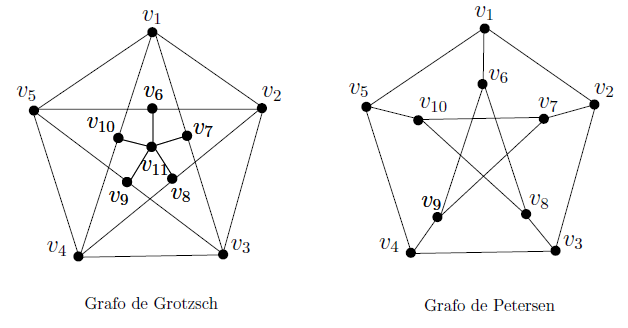
\includegraphics[scale=0.8]{Rel1}
\end{figure}
%
%\newpage
%
%\begin{ejercicio}{1.12}
%
%\end{ejercicio}
%\begin{solucion}
%
%\end{solucion}

\end{document}
